%====================================================%
% SEZIONE 1: Esercizi base
%====================================================%
\begin{question}[ID=1.1, subtitle={Automobile a velocità costante}, tags={mru, legge oraria}, difficulty=facile]
Un'automobile viaggia su una strada rettilinea con una velocità costante di $v = 20 \, \text{m/s}$. Supponi che l'auto mantenga questa velocità senza subire variazioni nel tempo.
\begin{enumerate}
    \item Quanto spazio percorre l'automobile in $t = 30 \, \text{s}$?
    \item Se il conducente guida per $2 \, \text{minuti}$, quanti chilometri avrà percorso al termine del viaggio?
\end{enumerate}
\begin{solution}
    \begin{enumerate}
        \item Lo spazio si calcola con la formula $s = vt$:
        \[
        s = 20 \cdot 30 = 600 \, \text{m}.
        \]
        \item Convertiamo il tempo in secondi: $2 \, \text{min} = 120 \, \text{s}$. Calcoliamo lo spazio:
        \[
        s = 20 \cdot 120 = 2400 \, \text{m} = 2{,}4 \, \text{km}.
        \]
    \end{enumerate}
\end{solution}
\end{question}

%------------------------------------------------------------------------------------%

\begin{question}[ID=1.2, subtitle={Treno passeggeri a 72 km/h}, tags={mru, conversione unità}, difficulty=facile]
Un treno passeggeri viaggia a velocità costante di $v = 72 \, \text{km/h}$ lungo un tratto rettilineo della ferrovia.
\begin{enumerate}
    \item Converti la velocità del treno in $\text{m/s}$.
    \item Calcola lo spazio percorso in $10 \, \text{minuti}$.
    \item Se il treno deve percorrere una tratta di $30 \, \text{km}$, quanto tempo impiegherà?
\end{enumerate}
\begin{solution}
    \begin{enumerate}
        \item La velocità in $\text{m/s}$ si ottiene dividendo per $3{,}6$:
        \[
        v = \frac{72}{3{,}6} = 20 \, \text{m/s}.
        \]
        \item Convertiamo $10 \, \text{min}$ in secondi: $600 \, \text{s}$. Lo spazio percorso è:
        \[
        s = 20 \cdot 600 = 12\,000 \, \text{m} = 12 \, \text{km}.
        \]
        \item Convertiamo $30 \, \text{km}$ in metri: $30\,000 \, \text{m}$. Il tempo si calcola con $t = s/v$:
        \[
        t = \frac{30\,000}{20} = 1500 \, \text{s} = 25 \, \text{min}.
        \]
    \end{enumerate}
\end{solution}
\end{question}

%------------------------------------------------------------------------------------%

\begin{question}[ID=1.3, subtitle={Velocità media del ciclista}, tags={mru, velocita media}, difficulty=facile]
Un ciclista percorre una strada pianeggiante a velocità costante. Dopo $15 \, \text{minuti}$, il contachilometri indica che ha coperto una distanza di $6 \, \text{km}$.
\begin{enumerate}
    \item Qual è la velocità media del ciclista espressa in $\text{m/s}$?
    \item Se mantiene la stessa velocità, quanto tempo impiegherà per percorrere $20 \, \text{km}$?
\end{enumerate}
\begin{solution}
    \begin{enumerate}
        \item Convertiamo: $t = 900 \, \text{s}$, $s = 6000 \, \text{m}$. La velocità media è:
        \[
        v = \frac{s}{t} = \frac{6000}{900} \approx 6{,}67 \, \text{m/s}.
        \]
        \item Per $s = 20\,000 \, \text{m}$:
        \[
        t = \frac{20\,000}{6{,}67} \approx 3000 \, \text{s} = 50 \, \text{min}.
        \]
    \end{enumerate}
\end{solution}
\end{question}

%------------------------------------------------------------------------------------%

\begin{question}[ID=1.4, subtitle={Atleta a velocità costante di 5 m/s}, tags={mru, legge oraria}, difficulty=facile]
Un atleta corre su un rettilineo mantenendo una velocità costante di $5 \, \text{m/s}$.
\begin{enumerate}
    \item Se l'atleta corre per $t = 12 \, \text{minuti}$ senza fermarsi, quale distanza avrà percorso?
    \item Dopo una pausa, l'atleta completa un tratto di $2 \, \text{km}$. Quanto tempo ha impiegato?
\end{enumerate}
\begin{solution}
    \begin{enumerate}
        \item Convertiamo: $t = 720 \, \text{s}$:
        \[
        s = 5 \cdot 720 = 3600 \, \text{m} = 3{,}6 \, \text{km}.
        \]
        \item Per $s = 2000 \, \text{m}$:
        \[
        t = \frac{2000}{5} = 400 \, \text{s} \approx 6{,}67 \, \text{min}.
        \]
    \end{enumerate}
\end{solution}
\end{question}

%------------------------------------------------------------------------------------%

\begin{question}[ID=1.5, subtitle={Traghetto tra due porti}, tags={mru, legge oraria}, difficulty=facile]
Un traghetto percorre un tratto rettilineo tra due porti distanti $15 \, \text{km}$ mantenendo $v = 25 \, \text{km/h}$.
\begin{enumerate}
    \item Quanto tempo impiega il traghetto per raggiungere il secondo porto?
    \item Se aumenta la velocità a $30 \, \text{km/h}$, quanto tempo risparmia?
\end{enumerate}
\begin{solution}
    \begin{enumerate}
        \item $t = s/v = 15/25 = 0{,}6 \, \text{h} = 36 \, \text{min}$.
        \item $t' = 15/30 = 0{,}5 \, \text{h} = 30 \, \text{min}$. Risparmio: $36 - 30 = 6 \, \text{min}$.
    \end{enumerate}
\end{solution}
\end{question}

%====================================================%
% SEZIONE 2: Quiz sul MRU
%====================================================%
\begin{question}[ID=2.1, subtitle={Grandezza costante nel MRU}, tags={mru}, difficulty=facile]
Quale grandezza rimane costante nel moto rettilineo uniforme?

\vspace{0.5em}

\begin{tabularx}{\linewidth}{@{}X X X X@{}}
\boxed{A}\hspace{6pt} la velocità &
\boxed{B}\hspace{6pt} l'accelerazione &
\boxed{C}\hspace{6pt} lo spazio &
\boxed{D}\hspace{6pt} il tempo
\end{tabularx}
\begin{solution}
Risposta: \textbf{A}. Nel MRU la velocità è costante per definizione; l'accelerazione è nulla (non costante e diversa da zero).
\end{solution}
\end{question}

\begin{question}[ID=2.2, subtitle={Unità di misura della velocità nel SI}, tags={mru}, difficulty=facile]
Qual è l'unità di misura della velocità nel Sistema Internazionale?

\vspace{0.5em}

\begin{tabularx}{\linewidth}{@{}X X X X@{}}
\boxed{A}\hspace{6pt} km/s &
\boxed{B}\hspace{6pt} km/h &
\boxed{C}\hspace{6pt} m/s &
\boxed{D}\hspace{6pt} m/s$^2$
\end{tabularx}
\begin{solution}
Risposta: \textbf{C}. L'unità SI della velocità è il metro al secondo (m/s).
\end{solution}
\end{question}

\begin{question}[ID=2.3, subtitle={Legge oraria del MRU}, tags={mru}, difficulty=facile]
Quale tra queste è la legge oraria del moto rettilineo uniforme?

\vspace{0.5em}

\begin{tabularx}{\linewidth}{@{}X X X X@{}}
\boxed{A}\hspace{6pt} $v = v_0 + at$ &
\boxed{B}\hspace{6pt} $s = s_0 + vt$ &
\boxed{C}\hspace{6pt} $s = s_0 + v_0t + \dfrac{1}{2}at^2$ &
\boxed{D}\hspace{6pt} $s = v_0t - \dfrac{1}{2}gt^2$
\end{tabularx}
\begin{solution}
Risposta: \textbf{B}. Nel MRU la posizione varia linearmente col tempo: $s = s_0 + vt$.
\end{solution}
\end{question}

\begin{question}[ID=2.4, subtitle={Grafico spazio-tempo del MRU}, tags={mru}, difficulty=facile]
Nel grafico spazio-tempo di un moto rettilineo uniforme, che funzione è rappresentata?

\vspace{0.5em}

\begin{tabularx}{\linewidth}{@{}X X X X@{}}
\boxed{A}\hspace{6pt} una retta &
\boxed{B}\hspace{6pt} una parabola &
\boxed{C}\hspace{6pt} una curva &
\boxed{D}\hspace{6pt} un punto
\end{tabularx}
\begin{solution}
Risposta: \textbf{A}. Poiché $s = s_0 + vt$ è una funzione lineare di $t$, il grafico $s$-$t$ è una retta con pendenza pari alla velocità.
\end{solution}
\end{question}

%====================================================%
% SEZIONE 3: Problemi di calcolo
%====================================================%
\begin{question}[ID=3.1, subtitle={Velocità media: 180 km in 2 h}, tags={mru, velocita media}, difficulty=facile]
Un'auto percorre 180 km in 2 h con velocità costante. Qual è la sua velocità in m/s?

\vspace{0.5em}

\begin{tabularx}{\linewidth}{@{}X X X X@{}}
\boxed{A}\hspace{6pt} 180 m/s &
\boxed{B}\hspace{6pt} 90 m/s &
\boxed{C}\hspace{6pt} 50 m/s &
\boxed{D}\hspace{6pt} 25 m/s
\end{tabularx}
\begin{solution}
Risposta: \textbf{D}. $v = 180\,\text{km}/2\,\text{h} = 90\,\text{km/h} = 90/3{,}6 = 25\,\text{m/s}$.
\end{solution}
\end{question}

\begin{question}[ID=3.2, subtitle={Velocità media su percorso in due tratti}, tags={mru, velocita media}, difficulty=facile]
In un viaggio di 90,0 km i primi 45,0 km vengono percorsi a 50,0 km/h e i restanti a 70,0 km/h. Determina la velocità media sull'intero percorso.

\vspace{0.5em}

\begin{tabularx}{\linewidth}{@{}X X X X@{}}
\boxed{A}\hspace{6pt} 50,3 km/h &
\boxed{B}\hspace{6pt} 60,0 km/h &
\boxed{C}\hspace{6pt} 58,3 km/h &
\boxed{D}\hspace{6pt} 68,3 km/h
\end{tabularx}
\begin{solution}
Risposta: \textbf{C}. $t_1 = 45/50 = 0{,}9\,\text{h}$; $t_2 = 45/70 \approx 0{,}643\,\text{h}$; $t_{tot} = 1{,}543\,\text{h}$;
$v_m = 90/1{,}543 \approx 58{,}3\,\text{km/h}$.
\end{solution}
\end{question}

\begin{question}[ID=3.3, subtitle={Spazio dalla legge oraria a t=5 s}, tags={mru, legge oraria}, difficulty=facile]
La legge oraria di un moto rettilineo uniforme è $s = 10 + 4{,}50\,t$ (s in metri, t in secondi). Qual è lo spazio percorso al tempo $t = 5{,}00\,\text{s}$?

\vspace{0.5em}

\begin{tabularx}{\linewidth}{@{}X X X X@{}}
\boxed{A}\hspace{6pt} 22,50 m &
\boxed{B}\hspace{6pt} 32,50 m &
\boxed{C}\hspace{6pt} 32,50 m/s &
\boxed{D}\hspace{6pt} Non si sa
\end{tabularx}
\begin{solution}
Risposta: \textbf{B}. $s = 10 + 4{,}50 \cdot 5{,}00 = 10 + 22{,}5 = 32{,}5\,\text{m}$.
\end{solution}
\end{question}

\begin{question}[ID=3.4, subtitle={Legge oraria del podista partito spostato}, tags={mru, legge oraria}, difficulty=facile]
Un podista parte spostato di 100 m dallo start e percorre 1000 m in 10 min e 20 s. Quale sarà la sua legge oraria?

\vspace{0.5em}

\begin{tabularx}{\linewidth}{@{}X X X X@{}}
\boxed{A}\hspace{6pt} $s = 10{,}20\,t$ &
\boxed{B}\hspace{6pt} $s = 100 + 1{,}02\,t$ &
\boxed{C}\hspace{6pt} $s = 1{,}61\,t$ &
\boxed{D}\hspace{6pt} $s = 100 + 1{,}61\,t$
\end{tabularx}
\begin{solution}
Risposta: \textbf{D}. $t = 10\,\text{min} + 20\,\text{s} = 620\,\text{s}$; $v = 1000/620 \approx 1{,}61\,\text{m/s}$; posizione iniziale $s_0 = 100\,\text{m}$.
\end{solution}
\end{question}

\begin{question}[ID=3.5, subtitle={Incontro tra due sistemi in moto sul grafico s-t}, tags={mru, grafico}, difficulty=media]
Considera il seguente grafico:
\begin{center}
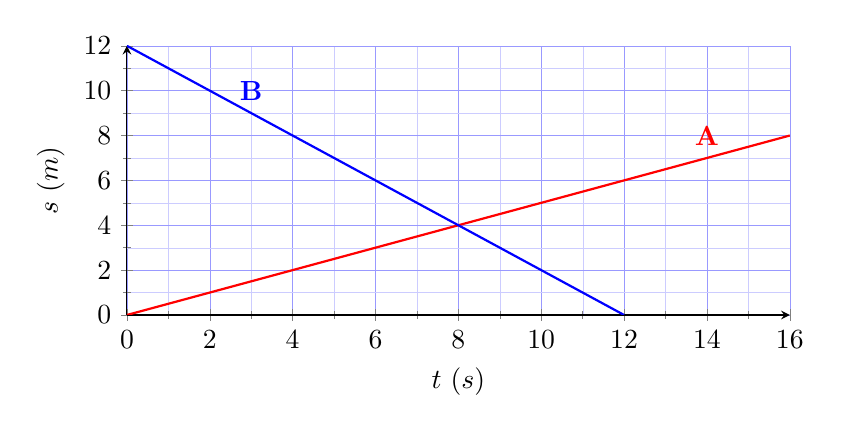
\begin{tikzpicture}
\begin{axis}[
    width=10cm,
    height=5cm,
    xmin=0, xmax=16,
    ymin=0, ymax=12,
    axis lines=left,
    xlabel={$t\ (\text{s})$},
    ylabel={$s\ (\text{m})$},
    xtick={0,2,4,6,8,10,12,14,16},
    ytick={0,2,4,6,8,10,12},
    grid=both,
    major grid style={line width=.2pt,draw=blue!40},
    minor grid style={line width=.1pt,draw=blue!20},
    minor tick num=1,
]
\addplot[red,thick,domain=0:16] {0.5*x};
\node[red] at (axis cs:14,8) {\textbf{A}};
\addplot[blue,thick,domain=0:12] {-x+12};
\node[blue] at (axis cs:3,10) {\textbf{B}};
\end{axis}
\end{tikzpicture}
\end{center}

\noindent
In che posizione si trova il sistema B al tempo $t = 4 \, \text{s}$?

\vspace{0.5em}

\begin{tabularx}{\linewidth}{@{}X X X X@{}}
\boxed{A}\hspace{6pt} 4 m &
\boxed{B}\hspace{6pt} 2 m &
\boxed{C}\hspace{6pt} 8 m &
\boxed{D}\hspace{6pt} Non si sa
\end{tabularx}

\vspace{1em}

\noindent
In che posizione si incontrano il sistema A e B?

\vspace{0.5em}

\begin{tabularx}{\linewidth}{@{}X X X X@{}}
\boxed{A}\hspace{6pt} 4 m &
\boxed{B}\hspace{6pt} 2 m &
\boxed{C}\hspace{6pt} 8 m &
\boxed{D}\hspace{6pt} Non si sa
\end{tabularx}

\vspace{1em}
\noindent
Scrivi le leggi orarie dei due sistemi:

\vspace{1em}

\begin{tabularx}{\linewidth}{@{}X X@{}}
Sistema A:\hspace{6pt} \rule{5cm}{0.2pt} &
Sistema B:\hspace{6pt} \rule{5cm}{0.2pt}
\end{tabularx}

\begin{solution}
\begin{enumerate}
    \item Posizione di B a $t=4\,\text{s}$: $s_B = -4 + 12 = 8\,\text{m}$ → Risposta: \textbf{C}.
    \item I sistemi si incontrano quando $s_A = s_B$:
    \[
    0{,}5t = -t + 12 \;\Rightarrow\; 1{,}5t = 12 \;\Rightarrow\; t = 8\,\text{s}, \quad s = 4\,\text{m}.
    \]
    Risposta: \textbf{A}.
    \item Leggi orarie: $s_A = 0{,}5\,t$;\quad $s_B = 12 - t$.
\end{enumerate}
\end{solution}
\end{question}
